\section{Key Parameters}

\begin{frame}{Stability and Accuracy}

    \textit{
        The second, symbol $s$, is the SI unit of time.
        It is defined by taking the fixed numerical value of the $Cs$ frequency $\Delta \nu_{Cs}$, the unperturbed ground-state hyperfine transition frequency of the $^{133}Cs$ atom, to be $9.192.631.770$ when expressed in the unit $Hz$, which is equal to $s^{-1}$.
    }

    \begin{figure}
        \centering
        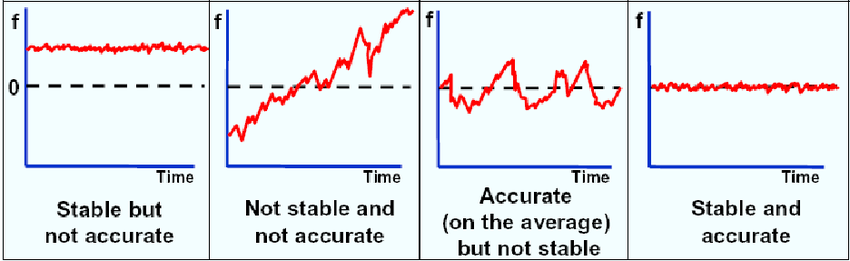
\includegraphics[width=0.9\textwidth]{img/stability-accuracy.png}
        % \caption{Accuracy and stability of an atomic clock.}
    \end{figure}

\end{frame}



\begin{frame}{Short term stability (Allan deviation $\sigma_y(\tau)$)}

    \begin{columns}[c, onlytextwidth]

        \begin{column}{0.5\textwidth}

            Allan deviation is a measure of the stability of a frequency standard.

            \begin{equation*}
                y(t) = \frac{f(t) - f_0}{f_0}
            \end{equation*}

            \begin{equation*}
                \sigma_y(\tau) = \sqrt{\frac{1}{2M} \sum_{i=2}^{M} (\bar{y}(\tau)_{i} - \bar{y}(\tau)_{i-1})^2}
            \end{equation*}

        \end{column}

        \hfill

        \begin{column}{0.45\textwidth}

            \begin{figure}
                \centering
                \only<1>{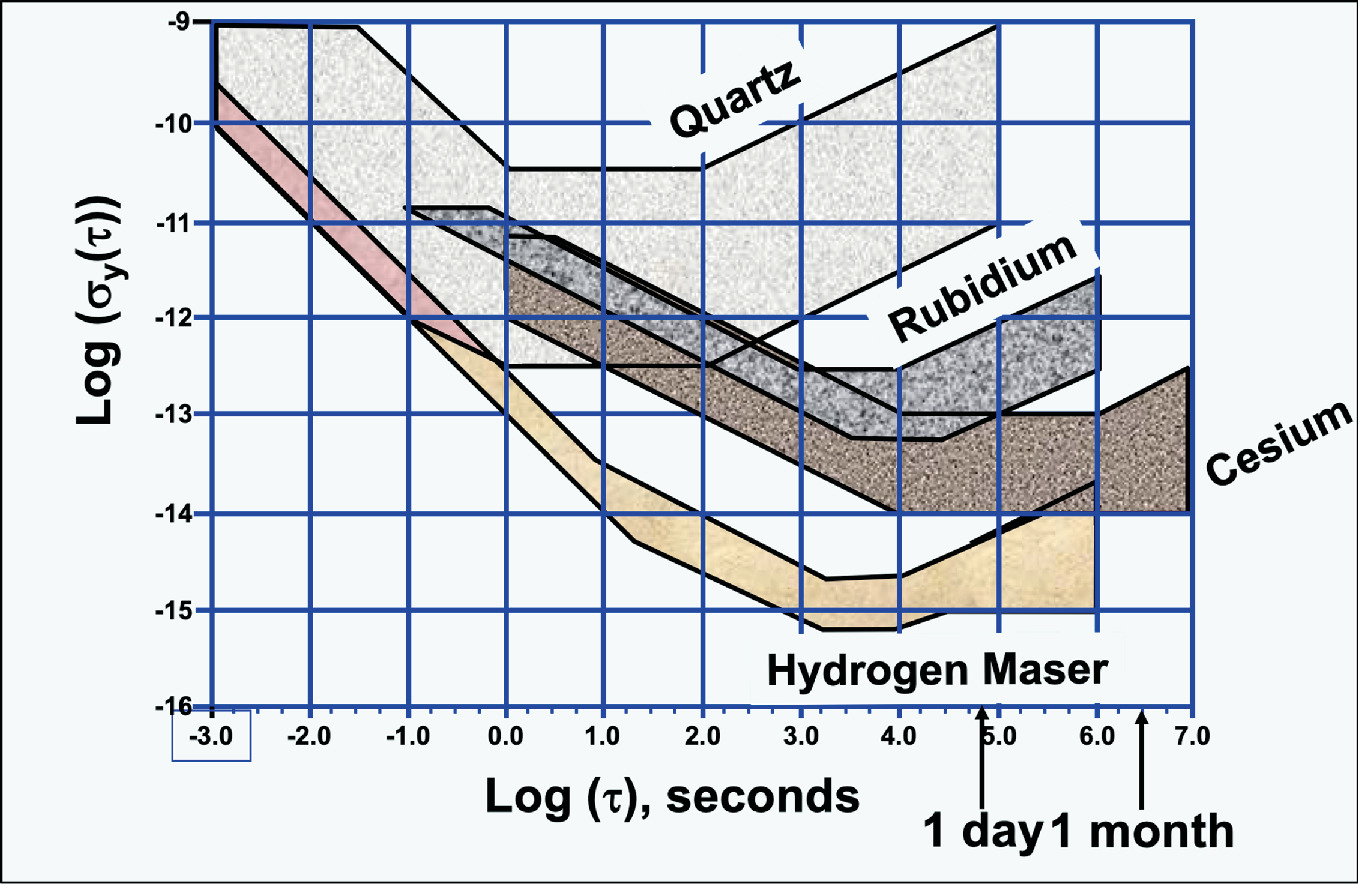
\includegraphics[width=\textwidth]{img/allan-with-quartz.png}}
                \only<2->{
                    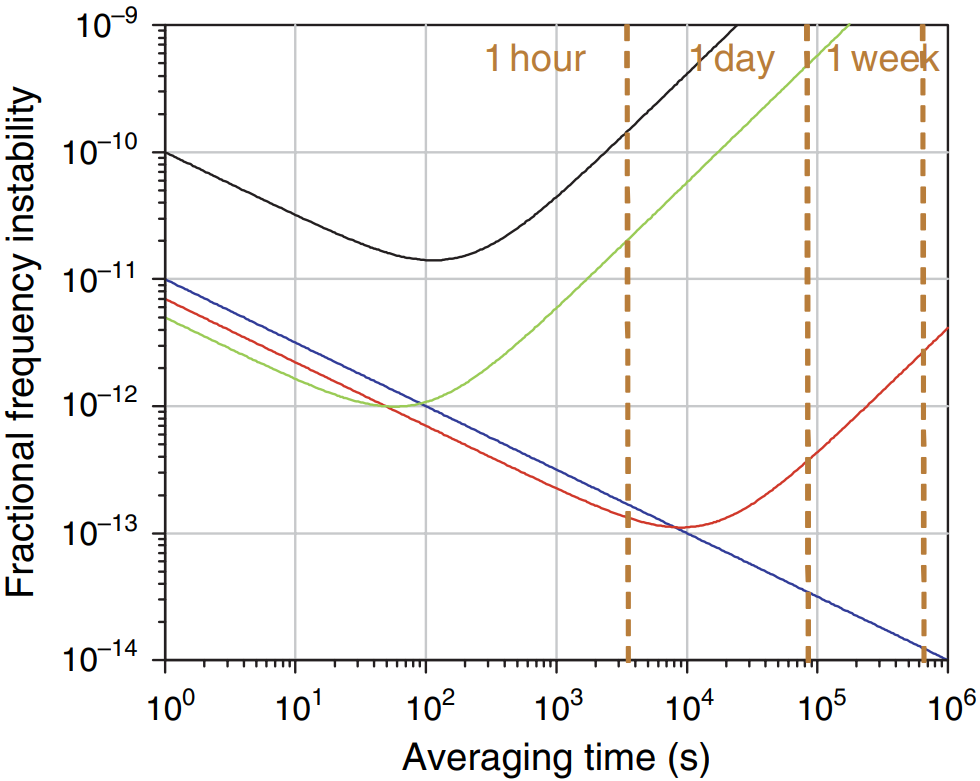
\includegraphics[width=\textwidth]{img/allan-without-quartz-2.png}
                    \caption{
                        \textcolor[HTML]{0000FF}{CBT},
                        \textcolor[HTML]{FF0000}{Rb},
                        \textcolor[HTML]{00FF00}{OCXO},
                        \textcolor[HTML]{000000}{TCXO}
                    }
                }
            \end{figure}

        \end{column}

    \end{columns}

    \only<1>{\vspace{10pt}}

    It captures the frequency \textbf{Fast Noise (mainly caused by the Local Oscillator (LO))} \& the Slow Drift (next slide)

    \footnotetext{
        $\sigma_y(\tau = 1s) = 3\times10^{-9}$ is equivalent to an instability in frequency between two observations 1 second apart with a (RMS) value of $3\times10^{-9}$.
        For a $10 MHz$ clock, this would be equivalent to $30 mHz$ RMS movement.
    }

\end{frame}



\begin{frame}{Medium term stability (Allan deviation $\sigma_y(\tau)$)}

    After the flicker floor, the \textbf{Slow Drift} became the dominant noise source and Allan deviation can be expressed as:

    \begin{equation}
        \sigma_y(\tau) = \frac{1}{Q\times SNR} \tau^{-1/2} \text{, where }
        \begin{cases}
            Q   \text{ Line quality}          & = \frac{\nu_0}{\Delta \nu}     \\
            SNR \text{ Signal-to-noise ratio} & = \frac{P_{signal}}{P_{noise}}
        \end{cases}
    \end{equation}

    \begin{columns}[c, onlytextwidth]

        \begin{column}{0.5\textwidth}

            \begin{figure}
                \centering
                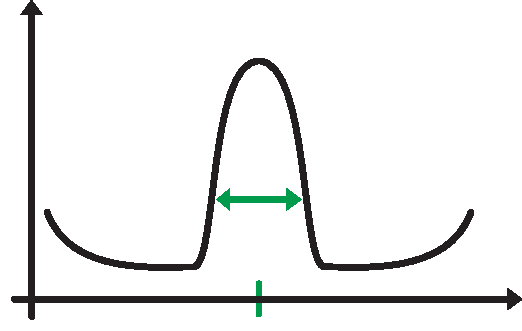
\includegraphics[width=0.7\textwidth]{pdf/Q-factor.pdf}
                \caption{$\nu_0$ and $\Delta \nu$.}
            \end{figure}

        \end{column}

        \begin{column}{0.5\textwidth}

            \begin{figure}
                \centering
                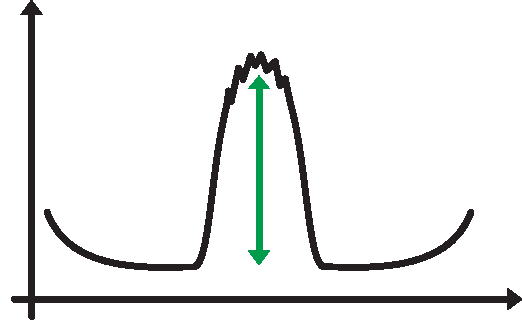
\includegraphics[width=0.7\textwidth]{pdf/P-signal.pdf}
                \caption{$P_{signal}$ and $P_{noise}$.}
            \end{figure}

        \end{column}

    \end{columns}

    \textbf{MODR}-based: lower $Q$ but higher $SNR$.\\
    \textbf{CPT}-based: higher $Q$ but lower $SNR$.

\end{frame}



\begin{frame}{Long term stability (Drift)}

    Drift is a measure of the long term stability of the clock which is caused by variation in the atomic reference frequency due to aging and environmental factors.

    \begin{figure}
        \centering
        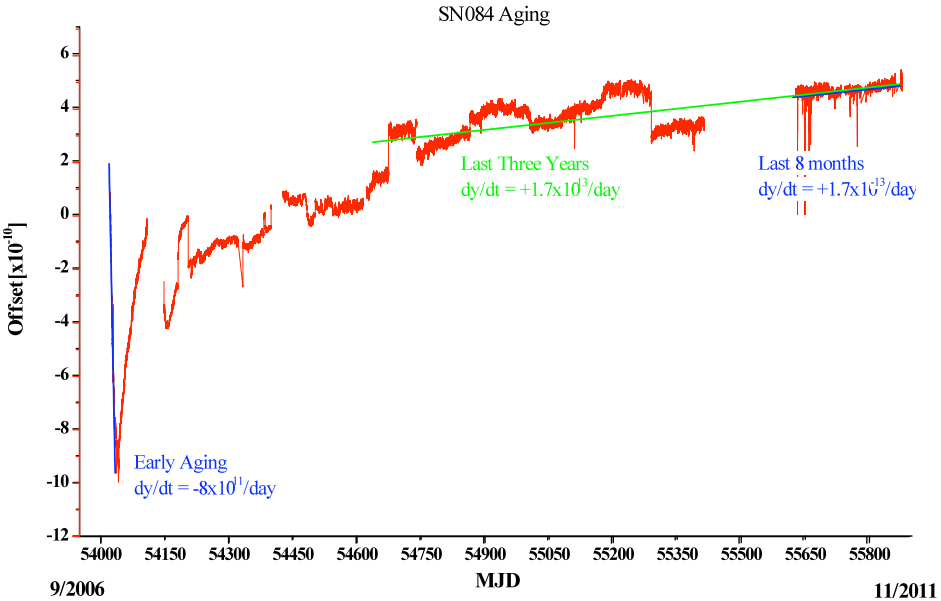
\includegraphics[width=0.7\textwidth]{img/drift.png}
        % \caption{Drift of an atomic clock.}
    \end{figure}

    % \footnotetext{Example: Drift of $10^{-10}$ means that the frequency of the oscillator changes by $10^{-10}$ per second.}
    \footnotetext{MJD: Modified Julian Dates, are a count of days since November 17, 1858.}

\end{frame}


% \begin{frame}{Thermal stability}

% \end{frame}